\documentclass[border=10pt]{standalone}
\usepackage{tikz}
\usetikzlibrary{arrows.meta, shapes.geometric, positioning, calc}

\begin{document}

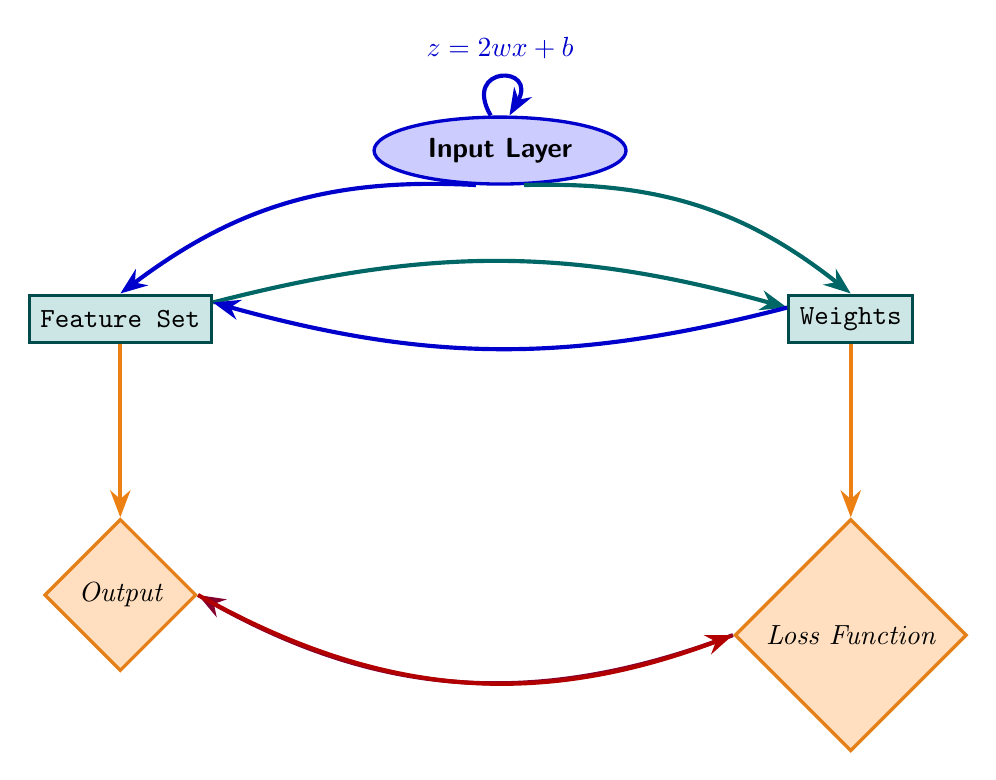
\begin{tikzpicture}[
    node distance=1.5cm and 2.5cm,
    base/.style={
        align=center,
        inner sep=4pt,
        minimum height=0.6cm,
        minimum width=1.2cm,
        line width=1.2pt
    },
    ellipse_node/.style={
        base,
        ellipse,
        font=\sffamily\bfseries,
        minimum height=0.85cm,
        minimum width=3.2cm,
        draw=blue!80!black,
        fill=blue!20
    },
    rect_node/.style={
        base,
        rectangle,
        font=\ttfamily,
        draw=teal!60!black,
        fill=teal!20
    },
    diamond_node/.style={
        base,
        diamond,
        font=\itshape,
        draw=orange!60!brown,
        fill=orange!25,
        aspect=1
    },
    arrow/.style={
        -Stealth,
        line width=1.5pt
    }
]

% Define colors for arrows
\colorlet{myblue}{blue!80!black}
\colorlet{myteal}{teal!80!black}
\colorlet{myorange}{orange!70!brown}
\colorlet{myred}{red!70!black}
\colorlet{mypurple}{purple!70!black}

% Place nodes
\node[ellipse_node] (input) {Input Layer};
\node[above=0.6cm of input, myblue] (eq) {$z = 2wx + b$};

\node[rect_node, below left=of input] (features) {Feature Set};
\node[rect_node, below right=of input] (weights) {Weights};

\node[diamond_node, below=2.2cm of features] (output) {Output};
\node[diamond_node, below=2.2cm of weights] (loss) {Loss Function};

% Draw arrows
% Top part and loop
\draw[arrow, myblue] (input.235) to[bend right=20] (features.north);
\draw[arrow, myteal] (input.305) to[bend left=20] (weights.north);
\draw[arrow, myblue] (input.105) to[out=120, in=60, looseness=8] (input.75);

% Middle horizontal arrows
\draw[arrow, myteal] (features.10) to[bend left=15] (weights.170);
\draw[arrow, myblue] (weights.170) to[bend left=15] (features.10);

% Vertical arrows
\draw[arrow, myorange] (features.south) -- (output.north);
\draw[arrow, myorange] (weights.south) -- (loss.north);

% Bottom part
\draw[arrow, mypurple] (loss.west) to[bend left=25] (output.east);
\draw[arrow, myred] (output.east) to[bend right=25] (loss.west);

\end{tikzpicture}

\end{document}
